% article_EN_4.0.tex — one-page presentation of WAC 4.0 for a DFIR magazine,
% English edition. The French edition is article_FR_4.0.tex, in this folder:
% both are maintained together, paragraph for paragraph. It follows the article
% on version 3.0 (article_EN_3.0.tex) and presents only what 4.0 adds.
%
% Build (LuaLaTeX, as the editor's recipe; build artefacts removed after):
%     ../build-docs.sh article/article_EN_4.0.tex
%
% Every figure comes from the validation and harmlessness files
% (doc/validation, doc/harmlessness) and the backlog, measured from 31 October
% to 4 November 2026 on the code of 4.0. Backlog B-061.

\documentclass[10pt,a4paper,twocolumn]{article}
\usepackage[english]{babel}
\usepackage{fontspec}
\setmainfont{Noto Sans}
\setmonofont{DejaVu Sans Mono}[Scale=0.84]
\usepackage[top=13mm,bottom=13mm,left=14mm,right=14mm,columnsep=7mm]{geometry}
\usepackage{xcolor}
\usepackage{titlesec}
\usepackage{enumitem}
\usepackage{array}
\usepackage{graphicx}
\usepackage{caption}
\captionsetup{font={small,color=gris},skip=2pt}
\usepackage[hidelinks]{hyperref}
\definecolor{marine}{HTML}{0A1A33}
\definecolor{bleu}{HTML}{2F6DB5}
\definecolor{gris}{HTML}{5B6573}
\pagestyle{empty}
\setlength{\parindent}{0pt}
\setlength{\parskip}{0.35em}
\titleformat{\section}{\color{marine}\normalsize\bfseries}{}{0em}{}
\titlespacing*{\section}{0pt}{0.7em}{0.2em}
\setlist{nosep,leftmargin=1.1em}
\newcommand{\wac}{\textsc{wac}}
\newcommand{\fichier}[1]{\texttt{#1}}
\hypersetup{pdftitle={WAC 4.0 — Windows servers, the directory and websites}}

\begin{document}

\twocolumn[{%
  {\color{marine}\LARGE\bfseries WAC 4.0: Windows servers, the directory and websites}\par
  \vspace{0.3em}
  {\color{gris}Aerospace Cyber Defence Centre of Excellence (CEC), French Air and Space Force Academy}\par
  \vspace{0.6em}
  {\itshape The articles on versions 2.0 and 3.0 presented \wac{} (Windows
  Artefacts Collector): a free collector, in C++, that reads volumes raw, writes
  nothing on the examined machine, and covers workstations from XP~SP1 to
  Windows~11. Version 4.0 moves on to servers: every generation from Server~2003
  to 2025, the directories of domain controllers, group policies and web
  servers.}\par
  \vspace{0.9em}
}]

\section{Every server, from 2003 to 2025}
The same executables collect Server~2003, 2008~R2, 2012, 2012~R2, 2016, 2019,
2022 and 2025, as well as Server~2022 as a Core installation. Each passed the
test cycle on the server itself, and that pass found what a workstation did not
show: a final LZX block of odd size that left \fichier{shell32.dll} half read,
older formats of Defender, and the ShimCache of Server~2003, now
decoded. Server~2008 without R2 is not measured, for want of an official image.

\section{The directory, without its secrets}
On a domain controller, \fichier{ntds.dit} and its logs are copied by raw reading,
with neither LDAP nor replication; the logs are replayed into the working copy,
because recent objects are only there. From it \wac{} draws each object, deleted
ones included, each value of a linked attribute with its removal date (who
entered a group, and who left), the replication metadata attribute by attribute,
and the security descriptors, where the rights of a DCSync attack can be read.
\textbf{Secrets are neither read nor written}: only a closed list of attributes
is decoded, and an attribute unknown to the schema stays unread. The copy of
\fichier{ntds.dit} holds them encrypted, and is protected as a hive is.

\section{Group policies}
\fichier{SYSVOL} is read the same way. For each policy: the registry values of
\fichier{Registry.pol}, scripts, scheduled tasks of the preferences, security
template. A password stored in a preference (\texttt{cpassword}) is flagged by
its file; its value is not written.

\section{Web servers}
IIS, Apache and nginx are found through their configuration and services: sites,
pools, modules, access and error logs, in UTC. Each site's folder is copied
whole, with any webshell it may hold. The connection strings of
\fichier{web.config} point to the databases to take; the accounts of SQLite
databases are drawn from them with the scheme of their hash (phpass, bcrypt, ASP.NET
Identity), and the data folders of MySQL, MariaDB and PostgreSQL are collected.
Not read: \fichier{wp-config.php} and \fichier{.env}.

\section{Checked against the live directory}
On a Server~2022 controller, the 3\,711 objects \wac{} returns are identical to
those of \texttt{Get-ADObject}. \wac{}'s ESE reader, set against
\texttt{dissect.esedb} on the same \fichier{ntds.dit}, gives 145\,421 values
without a single difference. Policies are checked against a witness policy, the
controller's events against \texttt{Get-WinEvent}. A replication request through
DirSync leaves a 4662 event for right \texttt{1131f6aa}, found in the collection.

\section{What remains to be measured}
The controller was tested only under Server~2022, alone in its forest, with no
real \texttt{sIDHistory}. Right \texttt{1131f6ad} of a true DCSync has no witness.
Server~2003's directory format is copied, not converted. On the controller,
Windows does not update access dates: the witness check of harmlessness proves
only the USN number there. The comparison with KAPE under Sysmon is still the
workstation one of 3.0.

\section{In figures}
\begin{tabular}{@{}>{\raggedright\arraybackslash}p{0.72\columnwidth}@{\hspace{0.5em}}r@{}}
Artefacts collected (3.0: 80) & 83 \\
Server generations measured & 2003 to 2025 \\
Checks in the cycle, domain controller & 571 \\
Checks in the cycle, Windows~11 & 582 \\
Directory objects identical to \texttt{Get-ADObject} & 3\,711 \\
\fichier{ntds.dit} values identical to dissect & 145\,421 \\
Directory secrets read or written & 0 \\
\end{tabular}

\section{Availability}
Version 4.0.0, Windows~XP~SP1 to 11 and Server~2003 to 2025 (x86 and x64), GPL~3.0
licence: \url{https://github.com/dev-cec/WAC}. Manuals, validation, harmlessness
and comparison files in French and English; server cycles from 31 October to
4 November 2026.

\vfill
\begin{center}
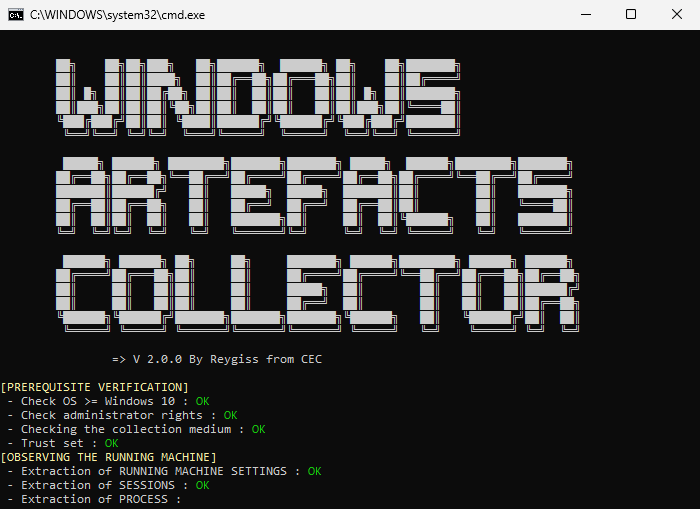
\includegraphics[width=\columnwidth,height=24mm,keepaspectratio]{../images/wac-running_EN.png}
\captionof*{figure}{\wac{} collecting.}
\end{center}

\end{document}
